\section{Управление VPS через Web-браузер}

OpenVZ Web Panel\footnote{OpenVZ Web Panel (OWP) разрабатывается Алексеем Южаковым и распространяется под лицензией GNU GPL v2.0}
представляет собой инструмент для управления серверами OpenVZ через веб-интерфейс. 
Основные особенности представлены ниже \cite{vzpanel}:
\begin{itemize}
    \item Интуитивно понятный интерфейс;
    \item Автоинсталлятор панели;
    \item Поддержка 10 языков интерфейса (в том числе русский и английский);
    \item Создание/удаление виртуальных серверов;
    \item Настройка лимитов виртуальных серверов (размер диска, объем памяти, лимиты на CPU);
    \item Возможность подключения нескольких физических серверов;
    \item Бэкап/восстановление виртуальных серверов;
    \item Клонирование виртуальных серверов;
    \item Быстрая переустановка виртуального сервера;
    \item Графики использования диска, памяти и процессора;
    \item Многопользовательская система с ролями.
\end{itemize}

Установка:
\begin{lstlisting}
# wget -O - http://ovz-web-panel.googlecode.com/svn/installer/ai.sh | sh
\end{lstlisting}

После установки, можно получить доступ к панели по адресу: \\
\texttt{http://IP\_address:3000}.

Логин/пароль по умолчанию: \texttt{admin/admin}.

\begin{figure}[ht]
	\begin{center}
	 	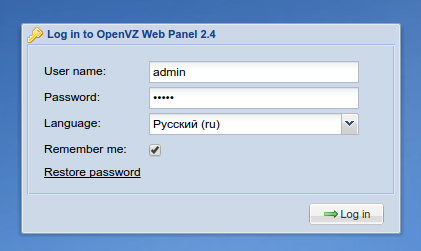
\includegraphics[width=0.6\linewidth]{vzpanel1.png}
	 	\caption{Вход в панель управления}\label{pic:vzpanel1}
	 \end{center}
\end{figure}

\begin{figure}[ht]
	\begin{center}
	 	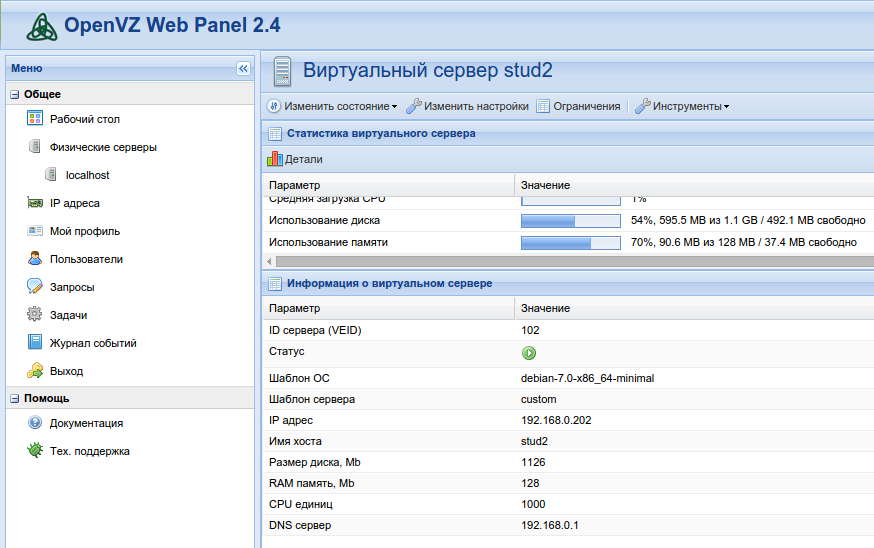
\includegraphics[width=0.7\linewidth]{vzpanel2.png}
	 	\caption{Информация о виртуальном сервере в OWP}\label{pic:vzpanel2}
	 \end{center}
\end{figure}

Приложение написано на Ruby, с использованием фреймворка Ruby on Rails. 
Также в проекте используются Ext JS\footnote{Ext JS "--- библиотека JavaScript для разработки веб-приложений и пользовательских интерфейсов}, и SQLite\footnote{SQLite "--- компактная встраиваемая реляционная база данных}. 

Всего за небольшой период разработки продукта, OWP обрела обширную аудиторию.
В версии 2.0 запланированы Remote API и интеграция с биллингом WHMCS.
Исходные файлы проекта в публичном доступе: \url{https://github.com/sibprogrammer/owp}

\clearpage
